\chapter{Introduction}

%=====================================================

% A introdução geral do documento pode ser apresentada através das seguintes seções: Desafio, Motivação, Proposta, Contribuição e Organização do documento (especificando o que será tratado em cada um dos capítulos). O Capítulo 1 não contém subseções\footnote{Ver o Capítulo \ref{cap-exemplos} para comentários e exemplos de subseções.}.


%=====================================================

As computers grow in power and shrink in size, more aspects of everyday life can be enhanced by adding processing units to common devices.
While many of these applications focus on conveniences, such as smart purchasing suggestions or automatic household control, computers can also be important to save time and save lives.
One way of achieving this is by adding computers and wireless transmitters to vehicles — such as cars, buses, and trains — so they can share data which may increase traffic efficiency or reduce the chance of accidents.

In 2013, an estimated 1.25 million people lost their lives due to traffic accidents globally \cite{whotraffic}.
While this number has greatly reduced over the past decades \cite{johnson2010traffic} fthanks to better safety features (seat belts, air bags, ABS, etc.) and stronger laws (drunk driving, motorcycle helmets, speed limits, etc.), it may still rise as a major cause of death in the years to come \cite{whofactsheet}, so further action is necessary.
Furthermore, as the car population increases, congestions consume ever more time of the daily commuter, peaking at over 100 hours per year for the residents of Los Angeles, CA \cite{inrixtraffic}.

Smart vehicles and vehicular networks are ways that technology can aid both of the aforementioned problems.
Through the use of sensors and wireless communications, these vehicles will be able to avoid accidents by alerting distracted drivers, or by knowing in advance another vehicle's position and speed.
By communicating, they can also collaborate to distribute traffic over alternative routes and, therefore, reduce the possibility of traffic jams.
These features are possible with the development of a vehicular ad-hoc network (VANET), in which vehicles can quickly share data amongst themselves without the need of a server or an Internet connection.

When dealing with safety or traffic-efficiency applications, it is crucial that network communications occur with low latency, which is why an ad-hoc solution is preferred.
Current technology could easily be used by connecting vehicles to the Internet through the cellular network, but the milliseconds added by the transmission could be enough to make certain applications unfeasible.
Cellular connections also have other problems: the connection would require an active subscription with a carrier; the connection depends on available infrastructure; the wireless frequency would be shared with phones and other mobile devices, increasing the possibility of interference and congestion; server-side issues could impact the vehicles' communications.

All these issues are solved by VANETs, since vehicles share data amongst themselves, using their own wireless transmitters, without having to rely on external devices.
Neighboring vehicles can share their position and velocity data at high frequencies, allowing, for example, autonomous vehicles to plan a platooning approach to traffic \cite{amoozadeh2015platoon}.
In the case of a collision or other event, nearby nodes can broadcast alerts, which other nodes will pick up and forward.
That way, an alert can travel long distances in little time, allowing approaching vehicles to safely slow down or pick alternative routes.

\begin{figure}[h]
    \centering
    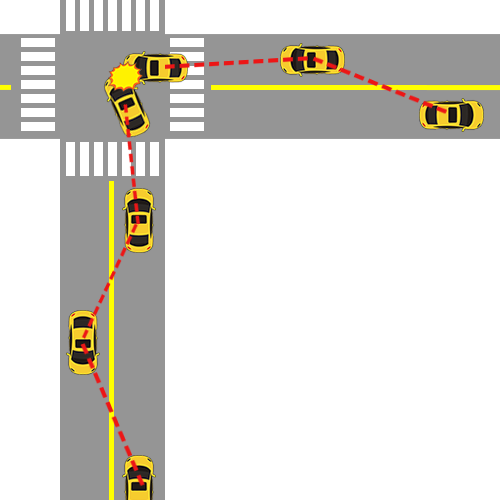
\includegraphics[width=0.5\textwidth]{images/collision.png}
    \caption{Propagation of a collision alert in a VANET}
    \label{fig:collision}
\end{figure}

However, as is the case for many types of networks, VANETs must be reliable in order to be functional.
In the case of ad-hoc networks, the nodes themselves must be reliable, since data can only propagate safely through benign cooperation.
Thus, the problem of trust arises in the context of vehicular networks.
Without trust management\footnote{There is an important distinction between \textit{trust} and \textit{trust management}.
The former relates to the actual trust relationship between a pair of nodes, while the latter concerns the management of previously generated trust data, such as previous tests or information received from neighboring nodes, and how this data can be used to make decisions.
While this work addresses trust management rather than trust itself, both terms will be used when referring to trust management for the sake of brevity.} features, a vehicle cannot judge whether or not received messages are benign or malicious in order to make an informed decision and, therefore, incorrect data might be presented to the driver.

Often, when people hear the term ``network'', they think only of technological examples, such as computer networks.
However, the study of complex networks dates back decades, including analysis of biological or social networks \cite{wang2003complex} \cite{newmannetworks}; technological networks, and VANETs by extension, are only a subset of that much larger field of study.

Trust issues and their solutions are an important aspect of the study of complex networks, and of social or technological networks in particular.
Each different type of network requires a specific approach to trust, according to the features that distinguish it from others, so it is interesting to review the solutions proposed for social networks and technological networks in general, in order to then narrow down on how dynamic networks, and VANETs in particular, are handled.
Despite the differences, there are some concepts that overlap across most types of networks.

This work proposes a method for identifying malicious nodes in a dynamic and decentralized network, using VANETs as a use-case scenario.
The solution is based on a previously existing algorithm \cite{vernize2015malicious}, which was limited to static networks.
In order to adapt the algorithm to a dynamic and decentralized environment, it is necessary to locate network features that allow for trust relationships to be developed amongst the network members over time, since there is no centralizing agent to store and process the whole network's trust values.
These features are found by tracing analogies to social networks, i.e. identifying how and why two nodes (in the case of VANETs, vehicles) would meet more than once and at a somewhat predictable interval.

%Further explain VANETs

%VANETs can be complex networks

%why mention social networks

\section{Document organization}
The remainder of this document is organized as follows:

\Cref{chap:complexnetworks} explains the broad study of complex networks and the importance of trust in technological and social networks.
Then, \cref{chap:vanets} goes into details regarding VANETs and the importance of trust solutions in the field, presenting previous studies made on the subject.
Finally, \cref{chap:proposal} shows the fundamentals of this proposed work, including the similarities found between VANETs and social networks, a realistic movement model that may be used for simulations, the previously existing study on malicious node identification for complex networks, and the important aspects that must be adapted to the dynamic vehicular environment.
